
%%%%%%%%%%%%%%%
%%%      CHAPTER      %%%
%%%%%%%%%%%%%%%

\chapter{Why do cells regulate? The fate of genetic regulation in an energy-limited cell's model}
\label{ch:part2:second_result}

\paragraph{}
\paragraph{}
\paragraph{}
\paragraph{}
\paragraph{}
\paragraph{}
\paragraph{}
\paragraph{}
\begin{center}
\large \textbf{The results presented in this chapter are preliminary and unpublished.}
\end{center}

%%%%%%%%%%%%%%%%%%%%%%%%% ABSTRACT %
\newpage

\paragraph{}
\begin{quote}
They are delighted he's going to eliminate regulations, let them make more profit; of course, it'll lead to another crash, but that's somebody else's problem.\\(Noam Chomsky, 2017)
\end{quote}

%%%%%%%%%%%%%%%%%%%%%%%%% SECTION : INTRODUCTION %

\section{Introduction}
\label{sec:part2:second_result:introduction}

While studied for decades, the role of genetic regulation in cellular functions and its evolution are still not completely understood \citep{savageau-1998,shinar-et-al-2006}. In living systems, many metabolic pathways are controlled by enzymes, whose expression levels are under regulation. The best known example of such a regulation is probably the lactose operon \citep{jacob-and-monod-1961}. When lactose is absent, the transcription of $\beta$-galactosidase, which degrades lactose in glucose and galactose, is repressed. When lactose is detected in the local environment, the repressor is inhibited, and $\beta$-galactosidase enzymes are produced.

It is often assumed that genetic regulation evolved to optimize cellular metabolism in variable environments. Many modeling tools in systems biology are based on this assumption. This is for example the case of \textbf{flux balance analysis} (FBA, \citealt{orth-et-al-2010}). FBA is based on mathematical optimization algorithms to find metabolic flux rates that maximize the production of one or more metabolites in a specific metabolic network, often linked to cellular fitness (\textit{e.g.} ATP production). FBA assumes that the cell is able to finely regulate its metabolic activity depending on some constraints (\textit{e.g.} the availability of a resource). For example, FBA has been used to study the evolution of cross-feeding in bacterial populations \citep{grosskopf-et-al-2016}.
Yet, this interpretation of the role of genetic regulation is undermined by recent works showing that ``\textit{the regulation of metabolic pathways may have evolved not to match expression of enzymes to levels of extracellular substrates in changing environments but rather to balance a trade-off between exploiting one type of nutrient over another}'' \citep{weisse-et-al-2015}. Indeed, living systems do not escape thermodynamic laws. Energy and resource allocation to various cell components are an essential limitation to cell's activity. \cite{weisse-et-al-2015} recently showed with an \textit{in silico} model of evolution that regulation may not evolve to adjust gene expression to external resource concentrations, but to balance internal trade-offs. Indeed, they showed that the best strategy in an environment providing a single nutrient is not to adjust gene expression to external nutrient concentrations, but to constitutively express enzymes to metabolize this nutrient at their maximum value, according to internal trade-offs. In environments providing two nutrients, the best strategy depends on the uptake efficiency of the cell for each nutrient. In this case, the expression level of enzymes metabolizing each nutrient only depends on relative uptake efficiencies, and not on external nutrient concentrations.

In {\EvoEvoSim}, genetic regulation, while freely evolvable, did not emerged in typical conditions, as shown in chapter \ref{ch:part2:first_result}. Indeed, in \cite{rocabert-et-al-2017}, the cell model is energy-free, meaning that regulation and metabolic networks evolve without any energy allocation trade-offs. In the complex situation of niche construction and the evolution of stable cross-feeding, none of the simulations shown evolved functional genetic regulation networks, while resource fluctuations were significant. The evolution of efficient metabolic pathways thus seems sufficient in these conditions to regulate the metabolic activity, without the intervention of genetic regulation.

In unpublished preliminary experiments with {\EvoEvoSim}, C. Knibbe initialized simulations with digital organisms owning carefully handcrafted regulation and metabolic networks, and undergoing energy constraints on their metabolism. She showed that even in tough environments and highly interdependent metabolic and regulation networks, digital organisms lost their regulation network and evolved a metabolic network with constitutively expressed enzymes. Moreover, organisms losing the regulation network had a better fitness than the ones keeping a finely regulated metabolism\footnote{This work has been presented to the \textit{Workshop of the International Laboratory EvoAct (Evolution in action)}, Autrans, April 2016.}. The study presented in this chapter is based on this preliminary work.

We first parameterized {\EvoEvoSim} with realistic values when it was possible, for two reasons: \textbf{(i)} it is impossible to explore the whole parameter space of {\EvoEvoSim}. We thus need an heuristic linked to our scientific question: in the case of an energy-limited model, realistic values are a good choice. \textbf{(ii)} {\EvoEvoSim} is a multi-scale model including the interaction of many objects and structures. To obtain appropriate results and avoid artifactitious dynamics, the different objects and structures must be parameterized in a coherent way. This can be done by setting all parameters in the same orders of magnitude as in real bacteria, when possible.

Using this parameter setting, we tested two specific environmental and cell model conditions. The first environment alternatively provides two resources: the metabolites \#20 and \#22. We called this environment \textbf{env. A}. We also ran a complementary experiment in a second type of environment (\textbf{env. B}), similar to the first one but providing more resources.
In the first model condition, the production of proteins costs energy. In the second one, this energetic cost is relaxed. However, in both conditions, pumping activity and anabolic reactions (\textit{i.e.} the production of metabolites with higher metabolite tag than the source metabolite, see chapter \ref{ch:part2:methodology}) consume energy, while catabolic reactions produce energy. Initial digital organisms own handcrafted genomes coding for carefully designed genetic regulation and metabolic networks (see below). When protein production energy costs exist, regulation is mandatory to survive, because it avoid the depletion of energy carrier molecules, as described below.

Our results show that the presence of protein production costs led to the evolution of ``virus-like'' organisms, having a small genome coding for a single operon, with no non-coding DNA. This operon codes for both regulation and metabolic networks. Doing so, digital organisms limit energy consumption in time by producing all proteins at once. In the absence of protein production costs, digital organisms evolved larger genomes with multiple small operons, half of the genome being non-coding. These organisms completely lost regulation. Thus, our results suggest that protein production costs strongly influence the evolution of genome structure and regulation in {\EvoEvoSim}. This preliminary work calls for further experiments in the model to assess the functional nature of genetic regulation.

%%%%%%%%%%%%%%%%%%%%%%%%% SECTION : METHODS %

\section{Methods}
\label{sec:part2:second_result:methods}

%%%%%%%%%%%%%%%%%%%%

\subsection{Realistic parameterization in {\EvoEvoSim}}
\label{subsec:part2:second_result:realistic_parameters}

\begin{quote}
\begin{center}
\textit{The section \ref{subsec:part2:second_result:realistic_parameters} is largely inspired from the final report of the EvoEvo project, available at \href{www.evoevo.eu}{www.evoevo.eu}.}
\end{center}
\end{quote}

{\EvoEvoSim} contains many parameters that must be set at the beginning of each simulation (chapter \ref{ch:part2:methodology} and Appendix \ref{ch:appendix:user_manual}). In the case of the study of internal cellular trade-offs, in order to compare the results of a simulation with \textit{in vivo} experiments, model parameters must be tuned to fit typical values found in living cells, for protein and metabolic concentrations, cellular lifespan, enzymatic constants, and so on. Moreover, since parameters are interdependent, one must set the correct order of magnitude of each parameter to avoid the emergence of purely artificial dynamics in the model. For example, metabolic reactions must be fast enough to enable the cell to react to environmental changes, but too fast reactions must be avoided since they would not be possible in practice. We identified the correct order of magnitude for most of the parameters of {\EvoEvoSim}. They are presented below.

\paragraph{$\bullet$ Time units.}
Parameters related to internal molecular processes were expressed per minute. At each simulation time-step and for each digital organism, the internal dynamics were computed by a time adaptive numerical solver (chapter \ref{ch:part2:methodology}) from $t=0$ to $t=100$ minutes. The population dynamics was thus updated every 100 minutes depending on the current state of each cell. Given this timescale, we fixed the death rate $p_{death}$ at 0.005 per organism per 100 minutes, meaning that each cell lives on average $\sim$14 days.

\paragraph{$\bullet$ Protein degradation rate.}
Proteins half-life in \textit{E. coli} vary from 2 minutes to 70 hours \citep{maurizi-1992}, depending on the protein (the proteins with low half-life generally being mutant or badly folded ones). In {\EvoEvoSim}, the protein half-life is fixed by the protein degradation rate $\phi$. We used a degradation rate $\phi$ of $5.10^{-4}$ per protein per minute, corresponding to a protein half-life of $\sim$24 hours.

\paragraph{$\bullet$ Protein concentration units.}
Following known values in model bacteria\footnote{For a global reference on the biological values, see \href{http://bionumbers.hms.harvard.edu/}{http://bionumbers.hms.harvard.edu/}.}, we fixed the cell volume and the grid patch volume to 4 $\mu$m\textsuperscript{3}, corresponding to the estimated volume of an \textit{E. coli} cell. In order to properly scale the concentrations, we chose the protein production rate as a relative reference. Let's first define the unit Z such that 1 Z = $10^{-8}$ M. In {\EvoEvoSim}, the protein production rate varies between 0 and 1. Given the protein degradation rate $\phi$, the maximum protein concentration at equilibrium is $1/5.10^{-4} = 2000$ Z. In \textit{E. coli}, enzymatic concentrations are estimated to vary between 5 and 500 nM. Hence, to fit these values, we considered that 1 Z was equal to $10^{-8}$ M, the protein concentrations thus varying between 0 and 20000 nmol/L. When a protein concentration is below than 1 Z, we consider that it has disappeared from the cell (since a concentration lower than 1 Z corresponds to less than one molecule in the cell).

\paragraph{$\bullet$ Metabolic concentration units.} 
In bacteria, intracellular concentration of metabolites varies between $10^{-7}$ and $10^{-2}$ M (\textit{i.e.}, $10$ to $10^{6}$ Z). Controlled environments used to cultivate \textit{E. coli} usually contain between 1 and 20 g/l of glucose, corresponding to metabolic concentrations of $5.10^{5}$ and $10^7$ Z in {\EvoEvoSim} (the minimal concentration below which \textit{E. coli} does not grow being 4$\sim$5 g/l).

\paragraph{$\bullet$ $K_M$ and $k_{cat}$ values.} 
$K_M$ and $k_{cat}$ are the two parameters of the Michaelis-Menten equation used in {\EvoEvoSim} to model the metabolic network dynamics. These values are encoded in the genome, are enzyme-specific and evolve freely. According to \cite{bar-even-et-al-2011}, in natural enzymes the observed values are usually between $10^{-7}$ and $10^{-1}$ M for $K_M$ ($10^1$ to $10^7$ Z), and between 6 and 60000 minute\textsuperscript{-1} for $k_{cat}$ (the median value being 600 minute\textsuperscript{-1}). Given the range of variation of both values, they are encoded in logarithmic scale, resulting in a range of 1 to 7 for $K_M$ and from 0.8 to 4.8 for $k_{cat}$.
However, these values raise an unanticipated difficulty: independent mutations on $K_M$ and $k_{cat}$ could result in a ratio $k_{cat}/K_M$ varying between $10^{-5.2}$ and $10^{2.8}$ min\textsuperscript{-1}Z\textsuperscript{-1}, which is a nonsense both mathematically (introducing artificial stiffness in ODEs) and biologically, since in natural enzymes, the $k_{cat}/K_M$ ratio varies between $6.10^{-4}$ and $6$ min\textsuperscript{-1}Z\textsuperscript{-1}. Indeed, a trade-off exists between $K_M$ and $k_{cat}$ values \citep{bar-even-et-al-2011}. We thus decided to parameterize the Michaelis-Menten reaction with two evolvable parameters: $k_{cat}$ and $k_{cat}/K_M$ ratio (see chapter \ref{ch:part2:methodology}). In consequence, in {\EvoEvoSim}, $k_{cat}$ varies between 0.8 and 3.8, with a median of 2.8. Compared to realistic values (0.8 to 4.8), we restrained the range of $k_{cat}$ to avoid very stiffed and intractable ODEs, but keeping the same median. The ratio $k_{cat}/K_M$ varies between -3.22 and -1.22.

Apart from the realistic parameterization, the dynamics of {\EvoEvoSim} model and the methodology used to solve ODE systems are exactly the ones presented in chapter \ref{ch:part2:methodology}. 

%%%%%%%%%%%%%%%%%%%%

\subsection{Initial handcrafted genome structure}
\label{subsec:part2:second_result:initial_genome_stucture}

For all the simulations in \textbf{env. A}, we initialized digital organisms with the same handcrafted genome. As shown in Figure \ref{fig:part2:second_result:initial_genome}, this genome contains two functional regions coding for two independent operons (\textbf{Op. 1} and \textbf{Op. 2}), each allowing for the production of an essential metabolite (respectively the essential metabolites \#5 and \#3), from two different external resources (respectively \#20 and \#22). 
As described in chapter \ref{ch:part2:methodology}, enzymatic reactions $\#20 \rightarrow \#5$ and $\#22 \rightarrow \#3$ are catabolic and provide energy to the cell, but pumps for \#20 and \#22 require energy. Each operon is self-inhibiting, unless its primary metabolite is present in the environment. To this aim, each operon encodes its self-repressing transcription factor (inhibited by its co-enzyme, the primary resource), a pump for the primary resource and an enzyme to convert it into an essential metabolite (\textit{i.e.} a prime number) (Fig. \ref{fig:part2:second_result:initial_genome}a). The corresponding metabolic pathways (\textbf{metabolic pathway 1} and \textbf{metabolic pathway 2}) are rather simple: each is dedicated to the production of an essential metabolite and each is regulated by an operon (Fig. \ref{fig:part2:second_result:initial_genome}b). In the case where protein production energy costs are high, this regulation scheme ensures a minimal energy consumption in the absence of the energy source. Indeed, we parameterized the protein production costs such that without such a self-inhibiting regulation pattern, digital organisms would die. The exact structure of the initial genome are shown in Table \ref{table:part2:second_result:initial_genome_structure}.

\begin{figure}
\centering
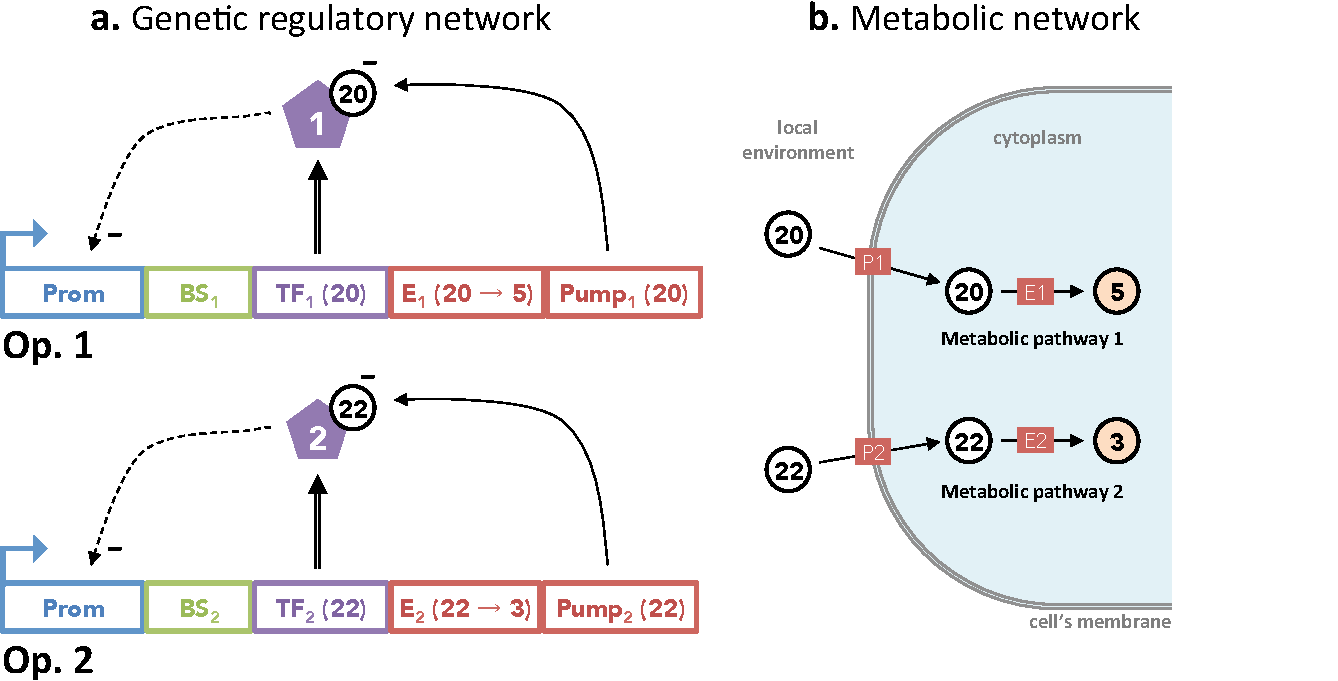
\includegraphics[width=1\textwidth]{part2_result2_initial_genome.pdf}
\caption[Initial handcrafted genome codes for two auto-repressed operons.]
{\textbf{Initial handcrafted genome codes for two auto-repressed operons.}
\textbf{a.} The initial handcrafted genome contains two independent operons \textbf{Op. 1} and \textbf{Op. 2}. Each operon (\textbf{Op. 1} or \textbf{Op. 2}). Both operons contain each a promoter (blue rectangle), an operator site composed of one binding site (green rectangles), a transcription factor coding unit (purple rectangles), and two enzyme coding units (red rectangles). $\text{TF}_1$ and $\text{TF}_2$ respectively encode transcription factors 1 and 2 (purple polygons) that repress their own expression (dashed arrow), except if they are inhibited by their co-enzyme (respectively metabolites \#20 and \#22). Thus, each operon is self-repressed in the absence of the co-enzyme.
\textbf{b.} Coding units $\text{E}_1$ and $\text{Pump}_1$ (respectively $\text{E}_2$ and $\text{Pump}_2$) encode two enzymes P1 and E1 (respectively P2 and E2), constituting \textbf{metabolic pathway 1} and \textbf{metabolic pathway 2}. Each metabolic pathway produces an essential metabolite (respectively the essential metabolites \#5 and \#3, dark circles filled in orange color), from two different external resources (respectively \#20 and \#22, dark circles), each being a co-enzyme of their respective transcription factor ($\text{TF}_1$ and $\text{TF}_2$). Thus, each operon is self-inhibiting, unless its primary metabolite is present in the environment.
}
\label{fig:part2:second_result:initial_genome}
\end{figure}

\begin{table}
\begin{adjustwidth}{-0in}{0in}
\centering
\caption[Initial genome structure.]{{\bf Initial genome structure.} In {\EvoEvoSim}, genomes are composed of \textbf{genetic units}, of five different types (promoters, binding sites, transcription factor coding units, enzyme coding units and non-coding units, see chapter \ref{ch:part2:methodology}). The genetic units used for generate the initial genome in this work are listed in the right order here (there is only one strand with a single reading frame in {\EvoEvoSim}). For all enzymes, $log_{10}(k_{cat})=2.8$ and $log_{10}(K_M/k_{cat})=-1.22$.}
%\resizebox{\textwidth}{!}{
\begin{tabular}{|l|c|c|c|}
\hline
Genetic unit type & Number & Main parameter values\\
\hline
\multicolumn{3}{|c|}{\textbf{Op. 1}}\\
\hline
Promoter & 1 & $\beta = 0.5$\\
Binding site & 1 & $\text{TF}_{tag} = 1$\\
Transcription factor & 1 & $\text{BS}_{tag} = 1$; $\text{coE}_{tag} = \#20$\\
Enzyme (pump) & 1 & $s=\#20$\\
Enzyme & 1 & $s=\#20$; $p=\#5$\\
Non-coding & 50 & --\\
\hline
\multicolumn{3}{|c|}{\textbf{Op. 2}}\\
\hline
Promoter & 1 & $\beta = 0.5$\\
Binding site & 2 & $\text{TF}_{tag} = 2$\\
Transcription factor & 2 & $\text{BS}_{tag} = 2$; $\text{coE}_{tag} = \#22$\\
Enzyme (pump) & 1 & $s=\#22$\\
Enzyme & 1 & $s=\#22$; $p=\#3$\\
Non-coding & 50 & --\\
\hline
\end{tabular}
%}
\label{table:part2:second_result:initial_genome_structure}
\end{adjustwidth}
\end{table}

%%%%%%%%%%%%%%%%%%%%

\subsection{Evaluation of the handcrafted digital organisms}
\label{subsec:part2:second_result:organisms_evaluation}

To evaluate our handcrafted genomes, we run simulations in \textbf{env. A} with null mutation rates, for 500,000 time-steps. We tested the two conditions cited above, namely with or without protein production energy costs, with 10 repetitions each. In \textbf{env. A}, two external metabolites (\#20 and \#22) are introduced at random in each environmental grid location, following a Poisson process $\mathcal{P}(\lambda)$, with $\lambda$ the introduction rate. In all simulations, $\lambda=0.01$ per location per time-step. The degradation rate $D_g$ is set to 0.0001 per gridspot per time-step in the first environment, and the diffusion rate $D$ is set to 0.01 per gridstep\textsuperscript{2} per timestep (a gridstep being the width of a gridspot).

The resulting typical cell's dynamics with protein production costs is shown in Figure \ref{fig:part2:second_result:dynamics}. The six panels display the behavior of a single cell through time, since its birth (one time-step corresponding to 100 minutes, see above). Each time one of the external resources (\#20 or \#22) is present in the local environment, the corresponding operon (\textbf{Op. 1} or \textbf{Op. 2}) produces the corresponding pump and enzyme (Fig. \ref{fig:part2:second_result:dynamics}a). The cytoplasm then contains the external resource (\#20 or \#22) that is transformed into the corresponding essential metabolite (\#5 or \#3) (Fig. \ref{fig:part2:second_result:dynamics}c). Each time an operon transcription is initialized, and before energy supply from the corresponding imported resource is sufficient, small drops in energy are visible due to temporarily unfavorable energy balance in the cell (Fig. \ref{fig:part2:second_result:dynamics}e black circles). The cell's score directly depends on the concentrations of essential metabolites (Fig. \ref{fig:part2:second_result:dynamics}f). At division, the tracked cell inherits half of protein and metabolite amounts of its mother, as clearly visible on Figure \ref{fig:part2:second_result:dynamics}b. Since cell's content is released in the environment at death, the concentration of cell's final products progressively increases in the environment (Fig. \ref{fig:part2:second_result:dynamics}d).

\begin{figure}[!h]
\centering
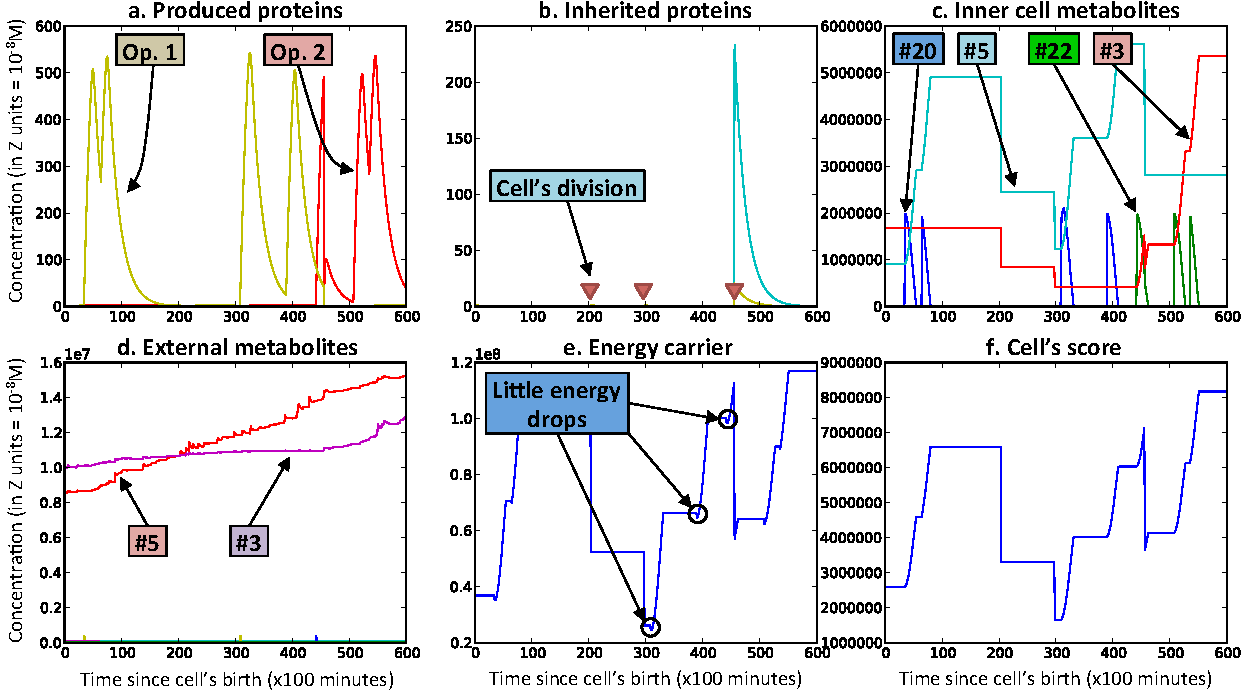
\includegraphics[width=1\textwidth]{part2_result2_dynamics.pdf}
\caption[Dynamics of initial digital organisms in environment A with null mutation rates.]
{\textbf{Dynamics of initial digital organisms in environment A with null mutation rates.}
The six panels display the behavior of a single cell through time, since its birth (one time-step corresponding to 100 minutes, see above). Each time one of the external resources (\#20 or \#22) is present in the local environment, the corresponding operon (\textbf{Op. 1} or \textbf{Op. 2}) produces the corresponding pump and enzyme \textbf{(panel a)}. The cytoplasm then contains the external resource (\#20 or \#22) that is transformed into the corresponding essential metabolite (\#5 or \#3) \textbf{(panel c)}. At the beginning of an operon transcription, and before energy is sufficiently produced by degrading the resource, small drops in energy are visible \textbf{(panel e black circles)}. The cell's score is directly dependent on the concentrations of essential metabolites \textbf{(panel f.)}. At division, the tracked cell inherits half of protein and metabolite amounts of its mother, as clearly visible on \textbf{panel b} (red triangles). Since cellular content is released in the environment at death, the concentration of cellular final products progressively increases in the environment \textbf{(panel d)}.
}
\label{fig:part2:second_result:dynamics}
\end{figure}

According to the cell's dynamics presented here, we were expecting that digital populations evolving in this conditions (env. A and null mutation rates) would never go to extinction. However, most of the simulations did not reach 500,000 time-steps. As shown on Figure \ref{fig:part2:second_result:extinction_nomut}, the extinction time was significantly higher (Wilcoxon-Mann-Whitney test gave a p-value of 0.017) for populations evolving without protein production costs (with a mean extinction time of 326,000t, 3 simulations out of 10 reached 500,000t), than populations evolving with protein production costs (mean extinction time of 160,000t, none of the simulations reached 500,000t). Two reasons explain these elevated extinction rate: \textbf{(i)} In environment A, external resources are provided at random, following a Poisson process. This could lead to prolonged periods of famine, possibly leading to whole population extinction, as it is surely the case for simulations without protein production costs. \textbf{(ii)} When protein production costs exist, energy drops at the beginning of each protein production (before the resource is sufficiently degraded to compensate for the associated energy cost) can lead to population's extinction, especially when energy level is already low (for example, after a cell division, or a prolonged famine, see Fig. \ref{fig:part2:second_result:dynamics}e). Thus, our handcrafted digital organisms are not very robust to environmental conditions as is, when no mutation occur in the genome. Extinctions occur especially early when protein production energy costs are applied (Fig. \ref{fig:part2:second_result:extinction_nomut}).

\begin{figure}[!h]
\centering
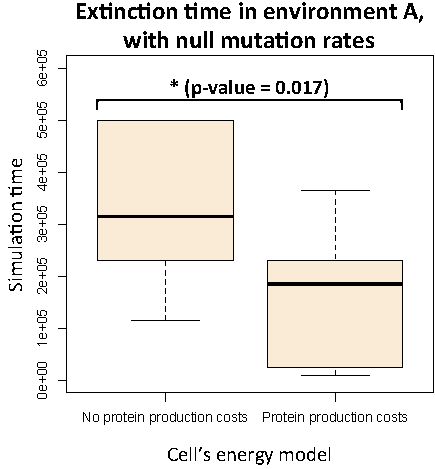
\includegraphics[width=0.5\textwidth]{part2_result2_extinction_nomut.pdf}
\caption[Extinction time in environment A with null mutation rates.]
{\textbf{Extinction time in environment A with null mutation rates.}
The dynamics of handcrafted digital organisms were tested in the environment A, with null mutation rates, and in both situations where protein production costs were imposed or not. The mean extinction time of populations evolving without protein production costs is 326,000 time-steps, 3 simulations out of 10 reaching the 500,000 time-steps. The extinction time of populations evolving with protein production costs is significantly lower (160,000t in mean), a Wilcoxon-Mann-Whitney test indicating a p-value of 0.017 (none of simulations reached 500,000t). The reasons of this elevated extinction rate are due to the cellular internal dynamics, and to the environmental variability, as explained above.}
\label{fig:part2:second_result:extinction_nomut}
\end{figure}

%%%%%%%%%%%%%%%%%%%%

\subsection{Experimental protocol}
\label{subsec:part2:second_result:experimental_protocol}

Based on the global parameter settings and the handcrafted genome presented above, we used {\EvoEvoSim} to run simulations in two different scenarios, with or without protein production energy costs.
\begin{enumerate}
\item[\textbf{(1)}] \textbf{Mutation rates.} {\EvoEvoSim} includes seven types of mutation rates (point mutation rate, duplications, deletions, inversions, translocations, breakpoints and type transitions, see chapter \ref{ch:part2:methodology}). They were all set to 0.01 (per attribute per replication for the point mutation rate, per genetic unit per replication for rearrangement and transition rates, and per attribute per breakpoint for the breakpoint rate)\footnote{We also run simulations with low mutation rates (all mutation rates being set at 0.001). However, the very low number of fixed mutations in evolved populations prevented any relevant analysis. We discussed this point in the discussion.};
\item[\textbf{(2)}] \textbf{Environment.}
The environment A described above was used in all simulations;
\item[\textbf{(3)}] \textbf{Protein production costs.}
In {\EvoEvoSim}, it is possible to set independent energy costs on each of the main activities of a cell (protein production, protein degradation, enzymatic reactions, pumps). For all the simulations, a positive cost were applied to enzymatic reactions and pumps (a cost of 1 Z of energy per Z of transformed, or pumped, metabolite). However, two costs were tested for the protein production: either an elevated cost (1000 Z per Z of produced proteins), or no cost at all (0 Z). The protein degradation cost was set to 0 for all the simulations;
\item[\textbf{(4)}] \textbf{Initial genomes.}
For all the simulations, we initialized digital organisms with the same handcrafted genome described above;
\item[\textbf{(5)}] \textbf{Simulation time.}
All the simulations have been run for 500,000 time-steps;
\end{enumerate}

We also tested a second environment (\textbf{env. B}), providing external resources ranging from \#20 to \#30. Environmental parameters were the same than for environment A, except that multiple resources could be provided at the same time. To compensate for the higher quantity of resource provided in the environment, the degradation rate $D_g$ was higher ($D_g=0.01$). In this environment, initial digital organisms own a handcrafted containing only one operon (\textbf{Op. 1}, see Fig. \ref{fig:part2:second_result:initial_genome}), in order to evaluate their capacity to innovate by creating new metabolic functions from their initial operon.

%%%%%%%%%%%%%%%%%%%%%%%%% SECTION : RESULTS %

\section{Results}
\label{sec:part2:second_result:results}

%%%%%%%%%%%%%%%%%%%%%%%%%

\subsection{Digital populations evolving under positive mutation rates are more robust to extinctions}
\label{subsec:part2:second_result:robust_extinction}

First, we evaluated the extinction time of populations evolving under positive mutation rates, compared to the test case with null mutation rates presented above. As shown on Figure \ref{fig:part2:second_result:extinction_withmut}, more populations were able to reach the 500,000 time-steps with mutations enabled than without, both without and with protein production energy costs.

Importantly, for technical reasons, we were not able to compute some simulations without protein production costs to the end. The main reason is the evolution of large metabolic networks in these simulations, with unseen dynamics in previous works with {\EvoEvoSim}. In some simulations, the time needed to finish the simulations (several months) would not have allowed us to conclude this chapter in reasonable delays. Hence, only 4 repetitions out of 10 in environment A without protein production costs were completed. They all reached 500,000 time-steps. Comparing these 4 simulations with the test case with a Wilcoxon-Mann-Whitney mean comparison test gives a p-value of 0.041, which is slightly significant.

For populations evolving with protein production costs, the Wilcoxon-Mann-Whitney mean comparison test is not significant (p-value of 0.623), even if 2 repetitions out of 10 reached 500,000 time-steps (other simulations went extinct).

Hence, evolution seems to allow digital organisms to fix mutation events that reduce the risk of extinction, thus making digital organisms more robust to famine episodes. In the next section, we will describe in more details the modifications undergone by the digital organisms, depending on the protein production energy costs. To this aim, we will focus on the simulations that reached the 500,000 time-steps.

\begin{figure}[!h]
\centering
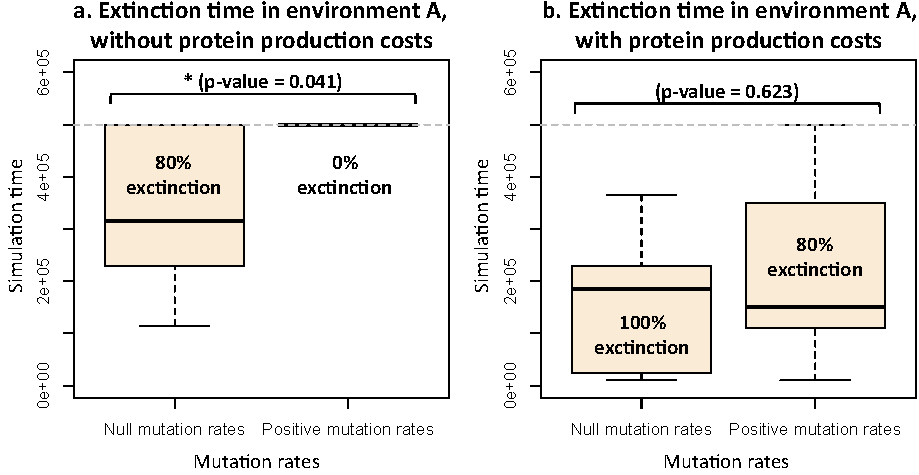
\includegraphics[width=1\textwidth]{part2_result2_extinction_withmut.pdf}
\caption[Extinction time in environment A.]
{\textbf{Extinction time in environment A.}
The dynamics of handcrafted digital organisms were tested in the environment A, with either null or positive mutation rates, and in both situations where protein production costs were imposed or not.
\textbf{a.} Extinction time without protein production costs. 80\% of the simulations went extinct with null mutation rates, while 0\% went extinct with positive mutation rates. A Wilcoxon-Mann-Whitney mean comparison test gives a p-value of 0.041, which is slightly significant.
\textbf{b.} Extinction time with protein production costs. 100\% of the simulations went extinct with null mutation rates, and 80\% went extinct with positive mutation rates. The Wilcoxon-Mann-Whitney mean comparison test is not significant.}
\label{fig:part2:second_result:extinction_withmut}
\end{figure}

%%%%%%%%%%%%%%%%%%%%%%%%%

\subsection{Digital populations without protein production cost lost regulation}
\label{subsec:part2:second_result:lose_regulation}

When mutation rates are enabled, for populations evolving with protein production costs, 2 repetitions reached 500,000 time-steps. For populations evolving without protein production costs, the 4 terminated repetitions reached 500,000 time-steps. The next results are based on these 6 simulations.

We evaluated the capacity of digital populations to keep their genetic regulation network through evolution. To this aim, we evaluated the last best individual (\textit{i.e.}, the individual having the best score, see chapter \ref{ch:part2:methodology}) of all simulations that reached the 500,000 time-steps, to see whether the genetic regulation network was lost or not.
If the last best individual possess a regulation network at the end of the simulation (even if it is different from the initial one), the organism was considered to have kept regulation. As shown in Table \ref{table:part2:second_result:keep_regulation_table}, digital organisms evolving in environment A without protein production cost (and with positive mutation rates) lost their regulation network in 7 repetitions out of 10 (Table \ref{table:part2:second_result:keep_regulation_table}). The 3 repetitions that kept regulation have non-functional networks. Thus, all the simulations evolving without protein production costs lost efficient regulation. On the contrary, all the populations evolving with protein production costs kept genetic regulation.

Thus, all the digital populations evolved towards a regulation-free metabolic network without internal energy trade-offs, their proteins being constitutively expressed. However, when significant internal trade-offs are introduced, by setting an energy cost to proteins production, all the simulations kept genetic regulation. This result is in agreement with \cite{weisse-et-al-2015}.

\begin{table}[!ht]
\begin{adjustwidth}{-0in}{0in}
\centering
\caption[Proportion of simulations that kept a regulation network.]{{\bf Proportion of simulations that kept a regulation network.} At the end of each simulation, if the last best individual had no regulation at all, the simulation was considered to have lost regulation.}
\begin{tabular}{|l|c|c|c|}
\hline
Scenario & Null mutation rates & Positive mutation rates\\
\hline
Env. A, no protein production cost & 100\% & 30\% (0\% functional)\\
Env. A, protein production cost & 100\% & 100\%\\
\hline
\end{tabular}
\label{table:part2:second_result:keep_regulation_table}
\end{adjustwidth}
\end{table}

%%%%%%%%%%%%%%%%%%%%%%%%%

\subsection{Protein production costs constrain the evolution of the genome structure}
\label{subsec:part2:second_result:genome_structure}

The results above suggest that the existence of internal cellular trade-offs (here an energy cost to the production of proteins) is a condition to at least keep, and possibly evolve genetic regulation networks. But what are the exact differences between digital organisms evolving with, or without protein production costs? One of the main advantage of \textit{in silico} experimental evolution is the possibility to get insights in the details of the structure of each organism. Using the same 6 simulations that reached 500,000 time-steps (4 without protein production costs, 2 with), we evaluated the structure of the last best individual of each simulation. We studied the structure of the genome, the regulation network, the metabolic network, as well as the metabolic content of the cytoplasm.

As shown in Table \ref{table:part2:second_result:genome_structure_table}, the genome structure evolved in very different directions depending on the presence or not of protein production costs. Indeed, populations evolving without production costs own bigger genomes, with many functional regions of small size, and a large proportion of non-coding DNA (except for repetition 8). However, populations evolving with production costs all evolved much smaller genomes, with a single functional region occupying almost 100\% of the genome. The latter population thus own a ``virus-like'' genome, with a single operon coding for all cellular functions. This situation is examplified in Figure \ref{fig:part2:second_result:genome_structure}, representing the genomes of the last best individuals of repetition 6 without protein production costs and of the repetition 2 with protein production costs. The single operon of the last best genome of repetition 2 is clearly visible (Fig. \ref{fig:part2:second_result:genome_structure}b), while 9 smaller operons are visible all along the last best genome of repetition 6 (Fig. \ref{fig:part2:second_result:genome_structure}a). Moreover, the latter genome does not contain any binding site (green triangles) and thus no regulation at all.

\begin{table}[!ht]
\begin{adjustwidth}{-0in}{0in}
\centering
\caption[Genome structure of the last best individuals in environment A.]{{\bf Genome structure of the last best individuals in environment A.} For each last best individual, we extracted the genome size, the proportion of coding sequences, the number of functional regions, and the mean size of functional regions. 4 genomes are evaluated without protein production costs, 2 with protein production costs.}
\resizebox{\textwidth}{!}{
\begin{tabular}{|c|c|c|c|c|}
\hline
Repetition & Genome size & Proportion of coding sequences & Nb. functional regions & Functional regions mean size\\
\hline
\multicolumn{5}{|c|}{\textbf{a. Without protein production costs}}\\
\hline
4 & 439 & 54.9\% & 58 & 4.16\\
5 & 282 & 66.7\% & 37 & 5.08\\
6 & 60 & 76.7\% & 9 & 5.11\\
8 & 30 & 100\% & 1 & 30\\
\hline
\multicolumn{5}{|c|}{\textbf{b. With protein production costs}}\\
\hline
2 & 32 & 90.6\% & 1 & 29\\
3 & 68 & 100\% & 1 & 68\\
\hline
\end{tabular}
}
\label{table:part2:second_result:genome_structure_table}
\end{adjustwidth}
\end{table}

\begin{figure}[!h]
\centering
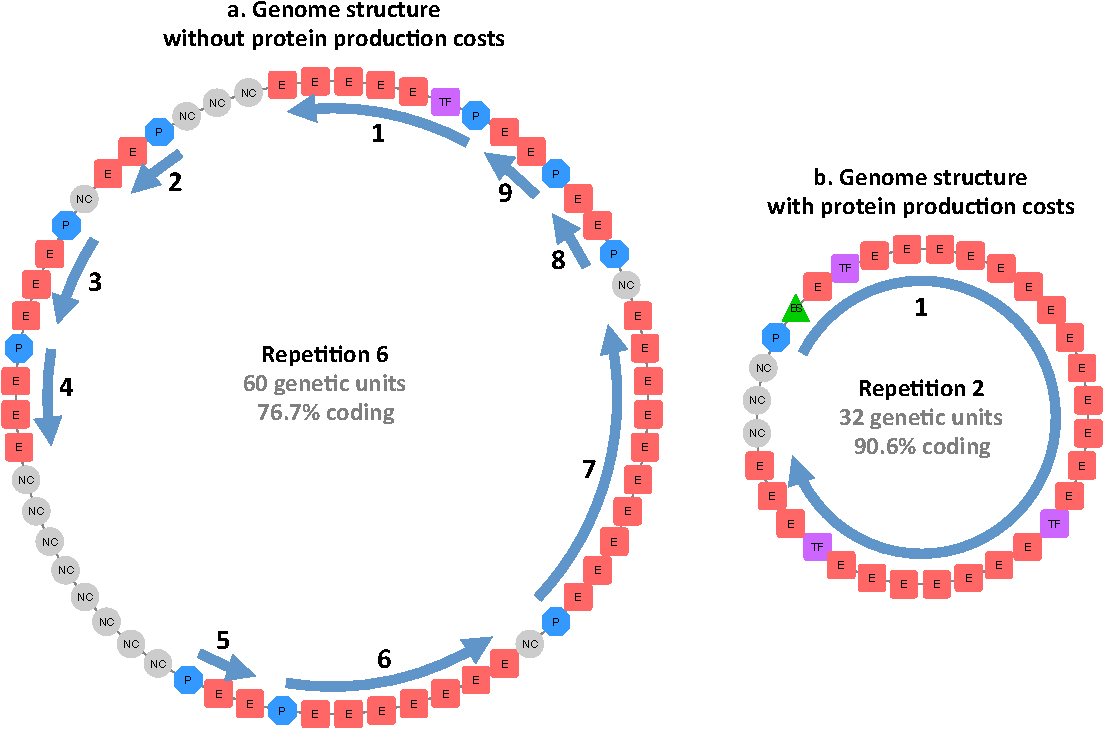
\includegraphics[width=1\textwidth]{part2_result2_genome_structure.pdf}
\caption[Two examples of evolved genome structures depending on protein production costs.]
{\textbf{Two examples of evolved genome structures depending on protein production costs.}
The genomes of the last best individuals of two examples are represented. Each functional region is indicated by a blue arrow. Grey circles: non-coding units (NC). Blue octagons: promoters (P). Green triangles: binding sites (BS). Purple squares: transcription factor coding units (TF). Red squares: enzyme coding units (E).
\textbf{a.} Last best individual's genome of the repetition 6 without protein production costs. $\sim$24\% of the genome is non-coding. 9 functional regions are visible, none of them having binding sites.
\textbf{b.} Last best individual's genome of the repetition 2 with protein production costs. $\sim$91\% of the genome is coding for a single operon owning an operator site.}
\label{fig:part2:second_result:genome_structure}
\end{figure}

%%%%%%%%%%%%%%%%%%%%%%%%%

\subsection{For digital populations evolving with protein production costs, reducing genome complexity enhances metabolic complexity}
\label{subsec:part2:second_result:genome_structure}

The analysis of the genome structure of populations evolving with protein production costs (Table \ref{table:part2:second_result:genome_structure_table} and Fig. \ref{fig:part2:second_result:genome_structure}b) indicates that the initial structure of the genetic regulation network has been modified in the course of evolution. Indeed, initial digital organisms owned two operons (as described above), while Table \ref{table:part2:second_result:genome_structure_table} indicates that evolved genomes own a single operon. In order to get more insights in this phenomenon, we recovered the lineage of the last best individual of the 2 repetitions that reached 500,000 time-steps and evaluated the main indicators of the evolution of the genome, the regulation network and the metabolic network. As show on Figure \ref{fig:part2:second_result:lineage} for repetition 2, the loss of a functional region leading to a ``virus-like'' genome (Fig. \ref{fig:part2:second_result:lineage}a red line) seems to allow for the evolution of more complex biochemical networks. Indeed, just after this important modification of the genome structure, the number of metabolic nodes and edges increased significantly all along evolution, as well as the functional genome size and the number of edges in the regulation network. Hence, the regulation network became smaller, but more connected, while the metabolic network globally grew. The situation is exactly the same for repetition 3 (data not shown).

\begin{figure}[!h]
\centering
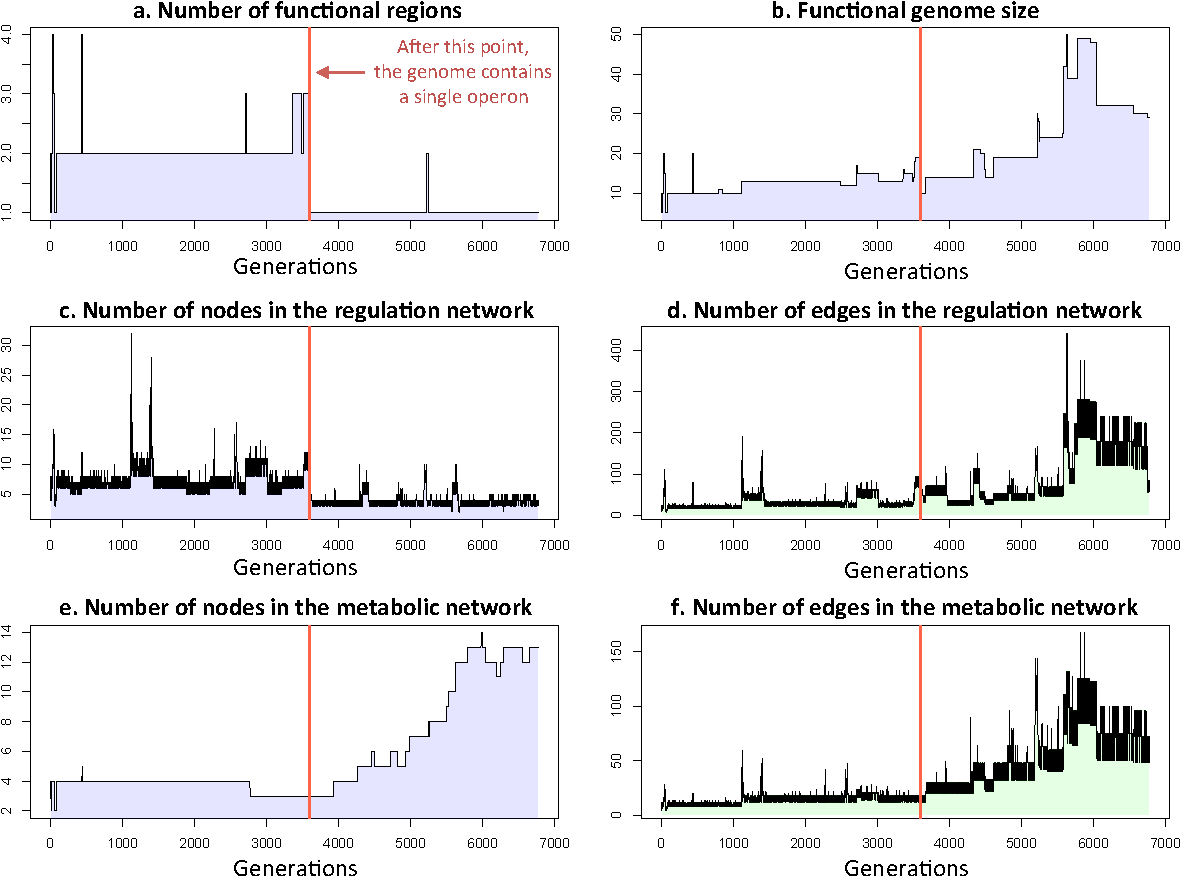
\includegraphics[width=1\textwidth]{part2_result2_lineage.pdf}
\caption[Evolution of genome and network structures in the lineage of an evolved organism in environment A with protein production costs.]
{\textbf{Evolution of genome and network structures in the lineage of an evolved organism in environment A with protein production costs.}
The lineage of the last best individual of the repetition 2 is recovered.
\textbf{a.} Evolution of the number of functional regions in the genome. Red line: at this point, the lineage undergone a genomic deletion and kept only one operon.
\textbf{b.} Evolution of the functional genome size (the genome size minus the non-coding DNA).
\textbf{c.} Evolution of the number of nodes in the genetic regulation network.
\textbf{d.} Evolution of the number of edges in the genetic regulation network.
\textbf{e.} Evolution of the number of nodes in the metabolic network.
\textbf{f.} Evolution of the number of edges in the metabolic network.
}
\label{fig:part2:second_result:lineage}
\end{figure}

Figure \ref{fig:part2:second_result:networks_example} shows the regulation network and the metabolic network corresponding to the last best individual of repetition 2. The structure of the genetic regulation network (Fig. \ref{fig:part2:second_result:networks_example}a) shows that a single transcription factor (purple rectangle at the center of the network) inhibits all the enzyme coding units. This transcription factor is repressed by co-enzyme \#20. The corresponding metabolic network (Fig. \ref{fig:part2:second_result:networks_example}b) is much more complex and connected than the initial metabolic network (see methods). 4 essential metabolites are produced (\#3, \#17, \#19 and \#23, red rectangles), from 6 different external resources (\#17, \#19, \#20, \#22, \#23 and \#26, blue rectangles). The environment A providing only external resources \#20 and \#22, other resources are wastes of population metabolic activity. Grey nodes correspond to non functional reactions. The properties of the last best individual of repetition 3 are similar (data not shown).

\begin{figure}[!h]
\centering
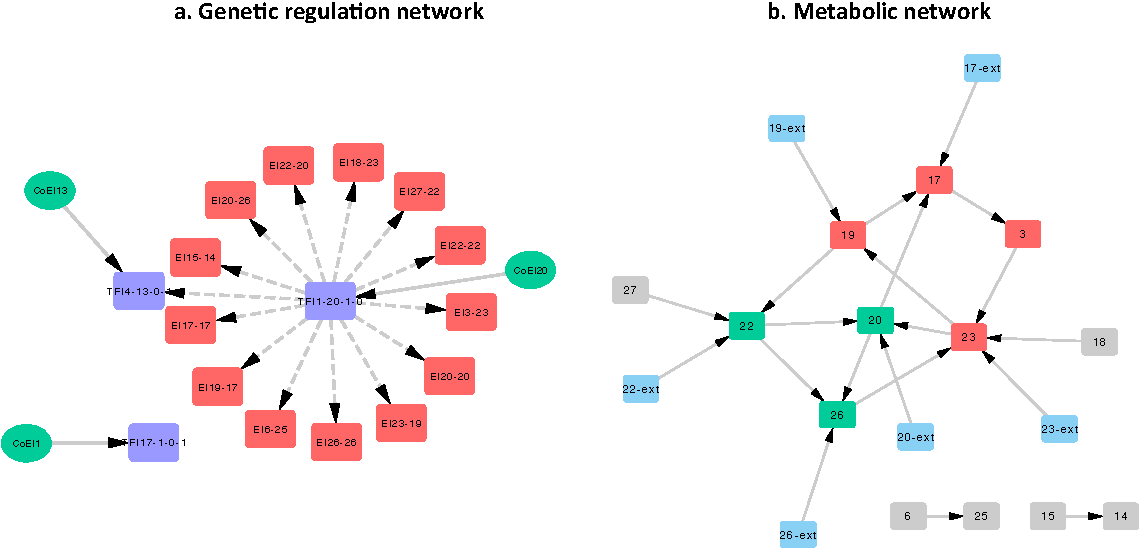
\includegraphics[width=1\textwidth]{part2_result2_networks_example.pdf}
\caption[Genetic regulation network and metabolic network of an evolved organism in environment A with protein production costs.]
{\textbf{Genetic regulation network and metabolic network of an evolved organism in environment A with protein production costs.}
The networks of the last best individual of the repetition 2 are represented.
\textbf{a.} Genetic regulation network. Green ellipses: co-enzymes (CoE|<metabolite tag>). Purple rectangles: transcription factors (TF|<BS tag; CoE tag; free activity; bound activity>, see chapter \ref{ch:part2:methodology}). Red rectangles: enzymes (E|<substrate; product>, see chapter \ref{ch:part2:methodology}). Solid arrows: positive regulation. Dashed arrows: negative regulation.
\textbf{b.} Metabolic network. Blue rectangles: external metabolite. Green rectangles: non-essential metabolites (see chapter \ref{ch:part2:methodology}). Red rectangles: essential metabolites (see chapter \ref{ch:part2:methodology}). Arrows: enzymatic reaction. 
}
\label{fig:part2:second_result:networks_example}
\end{figure}

Finally, looking at the metabolic content of the cytoplasm of the last best individual and at its local environment (Fig. \ref{fig:part2:second_result:cytoplasm}), we see that many metabolites are produced and released by digital organisms (at death since no outflowing pumps are coded in the genome). These cellular products are then available for other organisms, thus leading to a higher complexity of the metabolic network.

\begin{figure}[!h]
\centering
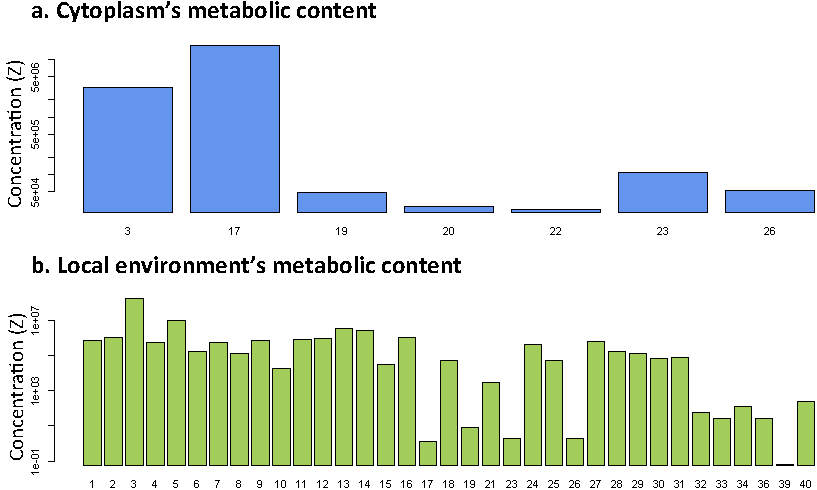
\includegraphics[width=0.8\textwidth]{part2_result2_cytoplasm.pdf}
\caption[Cytoplasmic metabolic content of an evolved organism in environment A with protein production costs.]
{\textbf{Cytoplasmic metabolic content of an evolved organism in environment A with protein production costs.}
\textbf{a.} List of metabolites present in the cytoplasm of the last best individual of repetition 2.
\textbf{b.} List of metabolites present in the local environment of this individual.}
\label{fig:part2:second_result:cytoplasm}
\end{figure}

%%%%%%%%%%%%%%%%%%%%%%%%%

\subsection{Digital populations evolving in diversified environments with protein production energy costs also evolved a single operon}
\label{subsec:part2:second_result:environment_B}

As presented above, we also evaluated our model with digital populations evolving in a second environment: environment B (see Methods). In this environment, multiple external resources are provided, ranging from metabolite \#20 to \#30. Thus, this environment is richer (many metabolites are provided at the same time) and more diversified than environment A. Initial digital organisms own a handcrafted genome only containing one operon: the \textbf{Op. 1} described above, that allows an organism to uptake metabolite \#20 and to produce essential metabolite \#5.

On the 10 populations that evolved in this environment, only two reached the 500,000 time-steps (repetitions 1 and 2)\footnote{The same simulations have been run with null mutation rates: 5 repetitions out of 10 reached 500,000 time-steps. The mean extinction time is 390,500 time-steps with no mutation, and 294,500 time-steps with positive mutation rates (a Wilcoxon-Mann-Whitney test gives a p-value of 0.152). Thus in the particular case of the environment B, it seems that digital organisms are more robust with null mutation rates, when they keep their initial structure. The reason is the abundance of external metabolite \#20, and thus the absence of prolonged famine. Evolving organisms are more exposed to whole population extinctions, meaning that evolution does not lead to more robust organisms in this case.}.
In the same manner than for the previous section, we evaluated in detail the structure of the last best individual of each repetition. As shown in Table \ref{table:part2:second_result:genome_structure_table_innovation}, final genomes present the same virus-like structure as for environment A with protein production costs, with only a single operon occupying the whole genome. However, in environment A, digital organisms had lost one operon (\textbf{Op. 2}), keeping and complexifying the remaining one (\textbf{Op. 1}). Coherently, in environment B, digital organisms kept their single operon.

\begin{table}[!ht]
\begin{adjustwidth}{-0in}{0in}
\centering
\caption[Genome structure of the last best individuals in environment B.]{{\bf Genome structure of the last best individuals in environment B.} For each last best individual, we extracted the genome size, the proportion of coding sequences, the number of functional regions, and the mean size of functional regions. 2 genomes are evaluated.}
\resizebox{\textwidth}{!}{
\begin{tabular}{|c|c|c|c|c|}
\hline
Repetition & Genome size & Proportion of coding sequences & Nb. functional regions & Functional regions mean size\\
\hline
1 & 11 & 100\% & 1 & 11\\
2 & 40 & 100\% & 1 & 40\\
\hline
\end{tabular}
}
\label{table:part2:second_result:genome_structure_table_innovation}
\end{adjustwidth}
\end{table}

However, as exemplified on Figure \ref{fig:part2:second_result:innovation_example} for the last best individual of the repetition 2, digital organisms evolved the ability to exploit the various resources provided in environment B, without losing the self-repressed regulation controlled by the co-enzyme metabolite \#20. Contrary to environment A, there is less chance for prolonged famine in environment B, since multiple resources are possibly provided at the same time at each environmental location. Thus, there is no particular reason to use the metabolite \#20 than any other in the environment, except for contingent historical reasons, independently from the environmental variability.

\begin{figure}[!h]
\centering
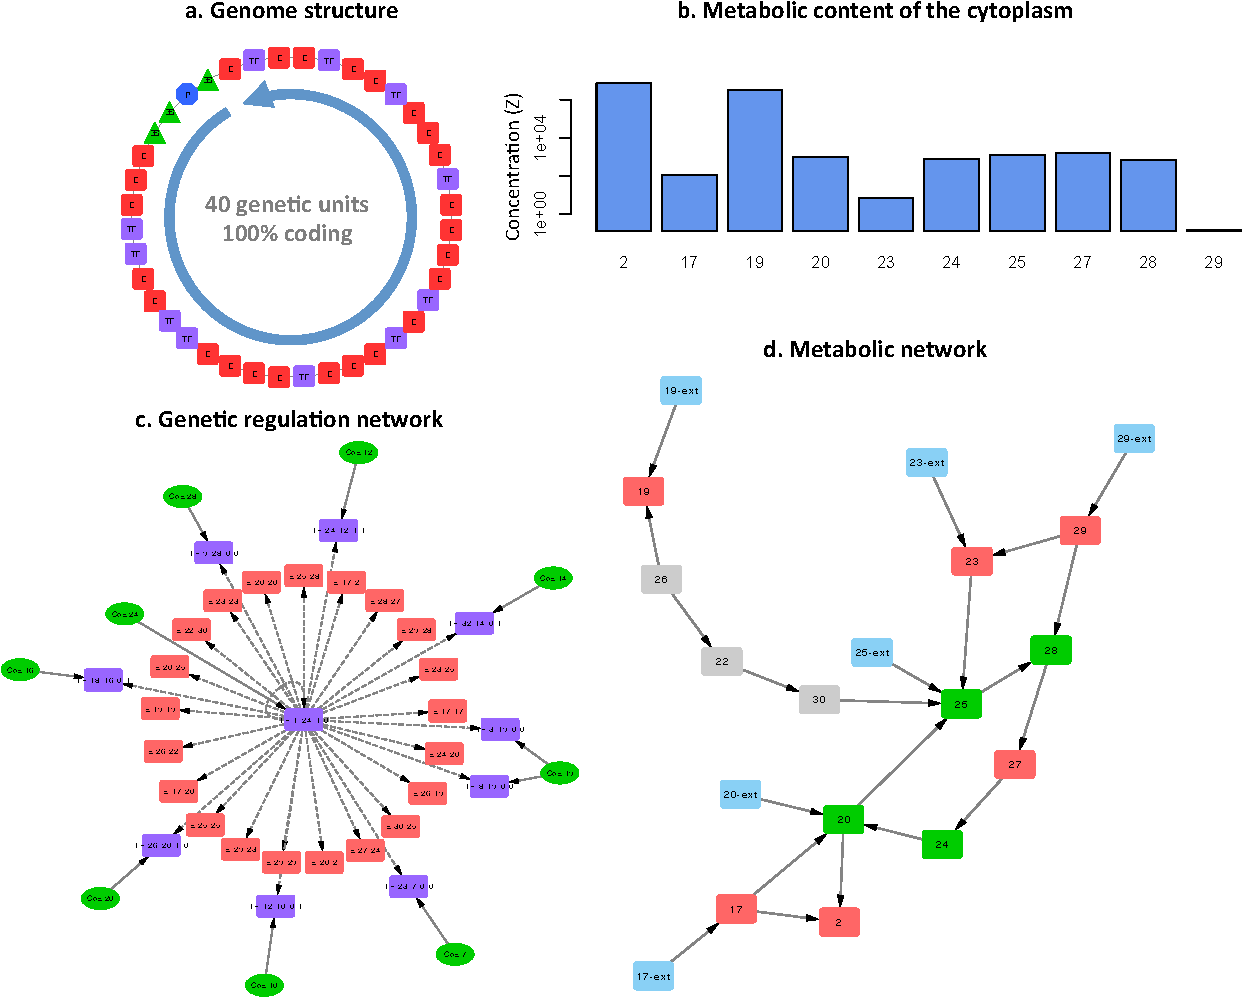
\includegraphics[width=1\textwidth]{part2_result2_innovation_example.pdf}
\caption[Structure of an evolved digital organism in environment B, with protein production costs.]
{\textbf{Structure of an evolved digital organism in environment B, with protein production costs.}
The structure of the last best individual of the repetition 2 is represented.
\textbf{a.} Genome structure. The single functional region is indicated by a blue arrow. Blue octagon: promoter (P). Green triangles: binding sites (BS). Purple squares: transcription factor coding units (TF). Red squares: enzyme coding units (E).
\textbf{b.} Cytoplasmic metabolic content. Concentrations are in arbitrary concentration units (ACU, see chapter \ref{ch:part2:methodology}).
\textbf{c.} Genetic regulation network. Green ellipses: co-enzymes (CoE|<metabolite tag>). Purple rectangles: transcription factors (TF|<BS tag; CoE tag; free activity; bound activity>, see chapter \ref{ch:part2:methodology}). Red rectangles: enzymes (E|<substrate; product>, see chapter \ref{ch:part2:methodology}). Solid arrows: positive regulation. Dashed arrows: negative regulation.
\textbf{d.} Metabolic network. Blue rectangles: external metabolite. Green rectangles: non-essential metabolites (see chapter \ref{ch:part2:methodology}). Red rectangles: essential metabolites (see chapter \ref{ch:part2:methodology}). Arrows: enzymatic reaction. 
}
\label{fig:part2:second_result:innovation_example}
\end{figure}

%%%%%%%%%%%%%%%%%%%%%%%% SECTION : DISCUSSION %

\section{Discussion}
\label{sec:part2:second_result:discussion}

Cellular metabolism is often considered to be finely tuned by the genetic regulation network by precisely adjusting enzymatic concentrations in response to environmental resource fluctuations.
However, as theoretically demonstrated by \cite{weisse-et-al-2015}, it seems that the role of genetic regulation is not to adapt the metabolic activity to environmental changes, but to balance internal energy and resource trade-offs.

In previous experiments with {\EvoEvoSim} \citep{rocabert-et-al-2017}, where the cell model was not energy-limited, no functional regulation network evolved (see chapter \ref{ch:part2:first_result}). In the attempt to study the maintenance and the evolution of genetic regulation, we parameterized {\EvoEvoSim} with realistic parameters values, and introduced strong energy trade-offs, by imposing energy costs to the main cellular functions (protein production, anabolism and active pumps). We then let digital organisms with handcrafted initial regulation and metabolic networks evolve in various conditions.

Although many simulations led to population extinctions, our preliminary results suggest that genetic regulation indeed evolved not to cope with environmental changes, but to balance internal energy trade-offs, and avoid premature cell death due to the depletion of energy carrier molecules (as suggested by \citealt{weisse-et-al-2015}). First, we showed that populations evolving without protein production costs lost genetic regulation, with no negative effect on the evolution of their metabolic network. On the contrary, populations that survive under strong protein production costs all kept regulation (Table \ref{table:part2:second_result:keep_regulation_table}). Moreover, our results showed that the genome structure of digital organisms evolving in {\EvoEvoSim} is strongly impacted by the existence of protein production costs: this includes the non-coding elements, while there is no cost to DNA replication in this model. Indeed, while digital populations without protein production costs evolved larger genomes, with a significant amount of non-coding DNA and many functional regions each coding for a few proteins, populations with protein production costs evolved compacted genomes, with no non-coding DNA and having a single functional region coding for a large operon. This self-repressed operon codes all the functions of the cell (regulation and metabolism), its expression being activated by single co-enzyme.

Digital populations evolving with protein production costs in diversified environments, providing more resources, also evolved this ``virus-like'' structure, with a single self-repressed operon, also activated by a single co-enzyme. This co-enzyme has no clear relation with environmental dynamics, but is the result of historical constraints and purely internal trade-offs, unlinked to environmental variability.

As a whole, our results suggest that in {\EvoEvoSim}, digital populations evolving with protein production energy costs undergo important constraints on their genome structure, while there is no cost to DNA replication. Indeed, such a ``virus-like'' structure could be a good way to limit energy consumption due to protein production, by expressing all cellular functions at a single time. This protein expression pattern could limit the number of energy drops. However, as shown on \ref{fig:part2:second_result:innovation_example}, this specific genome structure does not seem to limit the evolution of complexity, since digital organisms evolved in the diversified environment still exploit many resources.

As a next step, these preliminary results could be improved, at least in two directions:
\begin{enumerate}
\item[\textbf{(i)}] First, a parametric exploration should be performed on energy cost parameters and mutation rates. Indeed, in these simulations, we set the protein production costs such that digital organisms losing regulation under elevated protein production costs systematically die. Moreover, our energy model could be more realistic. In the current version of {\EvoEvoSim}, energy carrier molecules are not included in ordinary differential equations, and have no effect on reaction speed. It could be interesting to couple energy more intimately to the artificial chemistry of {\EvoEvoSim}, as it may provide more realistic cell's dynamics. In this work, we also run simulations with low mutation rates, but the very low number of mutation events fixed in those simulations prevented any relevant analysis. However, previous modeling and mathematical works suggested that mutation rates have a strong effect on the genome structure: populations evolving with high mutation rates own small genomes, with few non-coding DNA and large operons. On the contrary, populations evolving with low mutation rates own large genomes, with many non-coding DNA and many small operons \citep{knibbe-et-al-2007a,beslon-et-al-2010a,fischer-et-al-2014}. The relation between genome size and mutation rates follows a power law, linked to a long-term adjustment between the robustness and the evolvability of digital organisms. Thus, it could be interesting to study this effect in {\EvoEvoSim}, when high energy costs are applied. For example, by using {\aevol} software, \cite{knibbe-et-al-2007b} showed that a coupling exists between the amount of non-coding DNA and the deleteriousness of gene mutations. The more deleterious the gene mutations, the shorter the intergenic sequences (and thus the genome size). In this work, gene mutations are probably much more deleterious when protein production costs are applied, thus leading to smaller genomes with few non-coding DNA;
\item[\textbf{(ii)}] Second, a clear step is waiting to be crossed between these results and those from \cite{rocabert-et-al-2017} (see chapter \ref{ch:part2:first_result}). Indeed, the long-term evolution experiment (LTEE, \citealt{elena-and-lenski-2003}) provided insights in the evolution of stable cross-feeding \citep{rozen-et-al-2005}, but also in the evolution of genetic regulation and metabolic networks. In the LTEE, mutations that led to bacterial diversification in \textit{E. coli} are often linked to the regulation of metabolic pathways (see \textit{e.g.}, \citealt{grosskopf-et-al-2016}). Thus, replaying the experimental protocol from \cite{rocabert-et-al-2017} with more realistic parameters and energy costs could provide important insights in the understanding of bacterial diversification.
\end{enumerate}

Nonetheless, our preliminary results are in agreement with the work of \cite{weisse-et-al-2015}. Moreover, we were able to identify evolutive relationship between selective pressures at the level of the metabolism, and the structure of the genome. Even if the rationals of this relationship are still to be unraveled, this is a beautiful demonstration of the ability of multi-scale models to generate counter-intuitive outcomes, when multiple biological structures interact and evolve together.

% we evaluated the sigma position of symbiosis, catalysed by EMC-8pO which impulse the movements of Sigma-cell2D.


